\documentclass{article}
\usepackage{geometry}
\usepackage{tikz}
\usetikzlibrary{arrows.meta, matrix, positioning}

\newcommand\IntervalB[2]{%
\begin{tikzpicture}
    \draw[Stealth-Stealth] (-2.5,0) node[below]{$-\infty$} -- (2.5,0) node[below]{$\infty$};
    \draw[very thick,blue,{Bracket[#1,width=1.2em]}-{Bracket[#2,width=1.2em]}]
        (-1.5,0) node[above=4pt]{$a$} -- (1.5,0) node[above=4pt]{$b$};
\end{tikzpicture}
               }
\newcommand\IntervalR[2]{%
\begin{tikzpicture}
    \draw[Stealth-Stealth] (-2.5,0) node[below]{$-\infty$} -- (2.5,0) node[below]{$\infty$};
\ifnum#1=-1
    \draw[very thick,red,{Bracket[#2,width=1.2em]}-Stealth]
        (-1.5,0) node[above=4pt]{$a$} -- (2.5,0);
\else
    \draw[very thick,red,Stealth-){[#2,width=1.2em]}]
        (-2.5,0) -- (1.5,0)  node[above=4pt]{$b$};
\fi
\end{tikzpicture}
               }
\tikzset{matrixtable/.style = {%
    matrix of nodes,
     nodes={draw=blue, rounded corners=1ex,
            minimum height=3ex, inner ysep=1pt,
            top color=white,
            bottom color=blue!15,
            anchor=center},
    column sep=1ex,
    row sep=0.6ex,
    column 1/.style={text width=62mm,nodes={draw=red,bottom color=red!15}},
    column 2/.style={text width=17mm},
    column 3/.style={text width=56mm},
    row 1/.style={nodes={draw=red,bottom color=red!15}},
    draw, inner sep=1.5mm}}

\newsavebox\plotA
\newsavebox\plotB
\newsavebox\plotC
\sbox\plotA{\IntervalB{}{}}
\sbox\plotB{\IntervalB{}{reversed}}
\sbox\plotC{\IntervalB{reversed}{}}
%
\newsavebox\plotRA
\newsavebox\plotRB
\newsavebox\plotRC
\newsavebox\plotRD
\sbox\plotRA{\IntervalR{-1}{reversed}}
\sbox\plotRB{\IntervalR{-1}{}}
\sbox\plotRC{\IntervalR{1}{reversed}}
\sbox\plotRD{\IntervalR{1}{}}

\begin{document}
\begin{center}
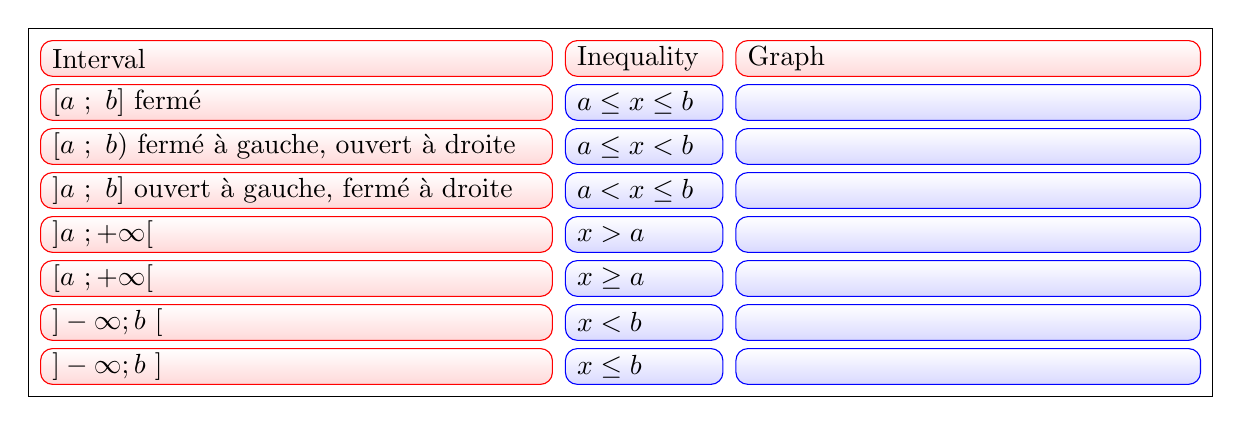
\begin{tikzpicture}
\matrix [matrixtable]
{
Interval     & Inequality      & Graph \\
$[a~;~b]$ fermé & $ a\le x\le b$    &   \usebox\plotA           \\
$[a~;~b)$ fermé à  gauche, ouvert à  droite
                & $a\le x<b $       &   \usebox\plotB           \\
$]a~;~b]$ ouvert à gauche, fermé à droite
                & $a<x\le b$        &   \usebox\plotC           \\
$]a~;+\infty [$ & $x>a$             &   \usebox\plotRA           \\
$[a~;+\infty [$ & $x\ge a$          &   \usebox\plotRB           \\
$]-\infty;b~ [$ & $x< b$            &   \usebox\plotRC           \\
$]-\infty;b~ ]$ & $x\le b$          &   \usebox\plotRD           \\
};
\end{tikzpicture}
\end{center}
\end{document}